\chapter{傅里叶、带宽与相干时间}
\label{chap:e02}

\begin{chapteropening}
上一章我们把光看成"一支飞快旋转的复振幅箭头"，也承认探测器太慢、只能记录被抹平后的强度。可是"太慢"到底相对于什么？光的相位又能维持多久不乱？要回答这些问题，得先学会一门通用的语言：任何一段波，无论多么复杂，都可以拆成一堆纯粹的单频正弦——就像一段和弦总能分解成一个个纯音。本章先把这门"拆音"的语言（傅里叶分析，Fourier analysis）讲清楚，再用它推出三个后面要反复用到的量：带宽 \(\Delta\nu\)、相干时间 \(\tau_c\)，以及把两者联系起来的自相关与功率谱。读完你会明白，为什么一个纳秒级的时间门里，其实塞进了成百上千个"相干时间"。
\end{chapteropening}

\section{任何波都是纯音的叠加}
\label{sec:e02-fourier-idea}

先建立画面。想象你手里有一段随时间变化的信号 \(f(t)\)：它可以是一根琴弦的位移，也可以是探测面上某一点的电场。傅里叶的洞见是：这段信号从来都不是"一整块"，而是许多不同频率的纯正弦波叠在一起的结果。低频的正弦画出大轮廓，高频的正弦补上尖锐的细节；把它们按各自的"份量"加起来，就还原出原信号。这份"每个频率占多少份量"的清单，就叫这个信号的\textbf{频谱}（spectrum）。

先看最容易想象的情形：信号是周期性的，周期为 \(T\)，也就是 \(f(t+T)=f(t)\)。这时候允许出现的频率不是连续的，而是一梯一梯的谐波：基频 \(\nu_1=1/T\)，以及它的整数倍 \(\nu_n=n/T\)。傅里叶级数（Fourier series）说，这样的周期信号可以写成
\begin{equation}
  f(t)=\sum_{n=-\infty}^{+\infty} c_n\,e^{\,i\,2\pi\nu_n t},
  \qquad
  \nu_n=\frac{n}{T},
  \label{eq:e02-fourier-series}
\end{equation}
\begin{formulaexplain}
\(f(t)\) 是周期为 \(T\) 的信号；\(\nu_n=n/T\) 是第 \(n\) 条谐波频率；复系数 \(c_n\) 是这条谐波在信号里所占的"份量"（含振幅与相位）。整条式子说：周期信号是一叠离散纯音之和。
\end{formulaexplain}
这里每一项 \(e^{i2\pi\nu_n t}\) 就是一支"以频率 \(\nu_n\) 匀速旋转的单位箭头"，复系数 \(c_n\) 决定这支箭头有多长（振幅）、初始指向哪里（相位）。由于 \(e^{i2\pi\nu_n t}\) 是无量纲的纯相位因子，信号 \(f(t)\) 的量纲便全部由复系数 \(c_n\) 承载；\(\nu_n\) 的单位是赫兹（\({\rm Hz}={\rm s^{-1}}\)）。要取出某一条谐波的份量，只需把信号和那条谐波"对一对拍子"——在一个周期内做积分，正交性会让其余谐波全部相消，只留下我们想要的一项：
\[
  c_n=\frac{1}{T}\int_{0}^{T} f(t)\,e^{-\,i\,2\pi\nu_n t}\,dt .
\]
其中用到的关键事实是不同谐波相互正交：\(\frac{1}{T}\int_0^T e^{i2\pi(m-n)t/T}\,dt=\delta_{mn}\)（当 \(m=n\) 时被积函数恒为 1，积分给 1；当 \(m\neq n\) 时是一个整周期的复指数，正负相消给 0）。这是我们第一次点名使用的"已知结果"，后面反复要用。

现在把周期 \(T\) 想象成越来越长。谐波的间隔 \(\Delta\nu=\nu_{n+1}-\nu_n=1/T\) 越来越密；当 \(T\to\infty\)，信号不再周期，一梯一梯的离散频率就融成一条连续的频率轴。这里最容易被跳过的一步是：级数里那个归一化因子 \(1/T\) 到底去哪了？把它交代清楚只需一个小技巧——在合成式 \eqref{eq:e02-fourier-series} 里给每一项配一个"频率间隔"因子 \(\Delta\nu\)（记住 \(\Delta\nu=1/T\)），乘一个再除一个，等式不变：
\[
  f(t)=\sum_{n} c_n\,e^{\,i2\pi\nu_n t}
      =\sum_{n} \frac{c_n}{\Delta\nu}\,e^{\,i2\pi\nu_n t}\,\Delta\nu .
\]
这一步什么也没改，只是把整条求和整理成了标准的黎曼和形状 \(\sum_n g(\nu_n)\,\Delta\nu\)——每一项都带着它所占的那一小格频率宽度 \(\Delta\nu\)。当 \(T\to\infty\) 时 \(\Delta\nu\to d\nu\)，黎曼和就收敛成积分，离散频率 \(\nu_n\) 变成连续变量 \(\nu\)，而括号里的组合 \(c_n/\Delta\nu\) 收敛到一条连续的\textbf{频谱密度}
\[
  \tilde f(\nu)\;=\;\frac{c_n}{\Delta\nu}\;=\;c_n\,T .
\]
于是 \(1/T\) 的下落就闭合了：它并没有凭空消失，而是被 \(\Delta\nu=1/T\) 吸收进了积分测度 \(d\nu\) 里，代价是频谱密度 \(\tilde f(\nu)\) 比原来的级数系数 \(c_n\) 大了整整 \(T\) 倍（这也和分析式对得上——把 \(c_n=\frac1T\int_0^T f\,e^{-i2\pi\nu_n t}dt\) 两边乘 \(T\)，右边的 \(1/T\) 正好消掉，留下的就是 \(\tilde f(\nu)=\int f\,e^{-i2\pi\nu t}dt\)）。这样求和 \(\sum_n\) 就干净地变成了积分 \(\int d\nu\)，我们也就从傅里叶级数过渡到了傅里叶变换（Fourier transform）。剩下的收敛数学细节我们不去纠缠，只保留这个物理直觉：非周期信号的频谱是连续的，每一个频率都可能出场，各自带着自己的份量。傅里叶变换对写成
\begin{equation}
  \tilde f(\nu)=\int_{-\infty}^{+\infty} f(t)\,e^{-\,i\,2\pi\nu t}\,dt,
  \qquad
  f(t)=\int_{-\infty}^{+\infty} \tilde f(\nu)\,e^{+\,i\,2\pi\nu t}\,d\nu .
  \label{eq:e02-fourier-transform}
\end{equation}
\begin{formulaexplain}
左式把时间信号 \(f(t)\) "拆"成频谱 \(\tilde f(\nu)\)；右式把频谱"合"回信号。\(e^{\mp i2\pi\nu t}\) 是频率为 \(\nu\) 的纯音。一拆一合互为逆运算，信息量不增不减。
\end{formulaexplain}
两式互为逆变换：左边（分析式）像用一排调好的音叉去"听"信号里每个频率有多强，右边（合成式）像把这些纯音按份量重新奏响、拼回原信号。要注意 \(\tilde f(\nu)\) 一般是复数：它的模 \(|\tilde f(\nu)|\) 说这个频率占多少份量，它的辐角说这个频率成分的相位。若把频率轴换成波长轴，这正是光谱仪吐出的那条谱线曲线的抽象版本。整本书后面谈"谱线宽度""滤光片带宽""相干函数"，底层用的都是这一对式子。

一句话小结：傅里叶变换是一台"拆音—合音"机器，把"随时间变化"翻译成"由哪些频率组成"。接下来我们让它干第一件真正有用的活。

\section{有限长的波包：时间越短，频率越宽}
\label{sec:e02-wavepacket}

真实的光从不是一列无限长、单一频率的完美正弦。恒星原子每发一次光，只辐射极短一小段波列就被碰撞打断；滤光片也只放行一小段频率。于是我们面对的总是\textbf{波包}（wave packet）：一段有头有尾、频率也不完全单一的振荡。这里藏着一条贯穿全书的铁律：\emph{一段波在时间上越短，它在频率上就越宽}；反过来，要频率极纯，就得让波列极长。

为什么？直觉是这样的：一列无限长的完美正弦，只需要一个频率就能描述，频谱是一根针。可一旦你把它"剪短"——乘上一个有限宽度的包络——就等于强行在两端把它掐灭，而"掐灭"这个动作本身需要额外的频率成分来完成（就像要奏出一个极短促的"哒"，必须动用很宽的一段音域）。波列越短，掐得越急，需要的频率越宽。用数量级写出来就是著名的
\begin{equation}
  \Delta\nu\,\Delta t \;\gtrsim\; 1 ,
  \label{eq:e02-bandwidth-time}
\end{equation}
\begin{formulaexplain}
\(\Delta t\) 是波包在时间上的持续宽度，\(\Delta\nu\) 是它在频率上的展宽。二者之积不能小于约 1：时间越窄，频率必然越宽。这是傅里叶变换的普适约束，不是仪器缺陷。
\end{formulaexplain}
式中 \(\Delta t\) 的单位是秒、\(\Delta\nu\) 的单位是赫兹，乘积无量纲。请注意这不是海森堡不确定性原理，而是纯经典波动性质；量子力学的 \(\Delta E\,\Delta t\gtrsim\hbar\) 只是把它乘上 \(E=h\nu\) 后的翻版。式 \eqref{eq:e02-bandwidth-time} 里的"\(\gtrsim\)"提醒我们它是量级关系，具体系数取决于怎样定义"宽度"和包络形状。下面就用一个能算到底的例子，把这条不等式变成等号。

\paragraph{高斯波包的显式计算}

取一个高斯包络调制的振荡，写成复数形式最省事：
\[
  f(t)=e^{-\,t^{2}/(2\sigma_t^{2})}\;e^{\,i\,2\pi\nu_0 t}.
\]
这里 \(\nu_0\) 是载波频率（可见光约 \(6\times10^{14}\,{\rm Hz}\)），\(\sigma_t\) 是包络的时间宽度（单位：秒）：\(|f|\) 在 \(t=0\) 达到峰值，在 \(|t|\sim\sigma_t\) 处衰减到峰值的 \(e^{-1/2}\)。我们来求它的频谱 \(\tilde f(\nu)\)。代入定义式 \eqref{eq:e02-fourier-transform}：
\[
  \tilde f(\nu)=\int_{-\infty}^{+\infty}
  e^{-\,t^{2}/(2\sigma_t^{2})}\,e^{\,i\,2\pi\nu_0 t}\,e^{-\,i\,2\pi\nu t}\,dt
  =\int_{-\infty}^{+\infty}
  e^{-\,t^{2}/(2\sigma_t^{2})}\,e^{-\,i\,2\pi(\nu-\nu_0)t}\,dt .
\]
把指数并成"二次型 + 一次项"的标准形式，令 \(a=\dfrac{1}{2\sigma_t^{2}}\)、\(b=i\,2\pi(\nu-\nu_0)\)，被积函数是 \(e^{-a t^{2}-b t}\)。这里要点名使用一个已知结果——\textbf{高斯积分}的配方公式：
\[
  \int_{-\infty}^{+\infty} e^{-a t^{2}-b t}\,dt
  =\sqrt{\frac{\pi}{a}}\;e^{\,b^{2}/(4a)},
  \qquad(a>0).
\]
（它的来路是把指数配方成 \(-a(t+\tfrac{b}{2a})^2+\tfrac{b^2}{4a}\)，再用最基本的 \(\int e^{-a u^2}du=\sqrt{\pi/a}\)。）代入 \(a,b\)：
\[
  \sqrt{\frac{\pi}{a}}=\sqrt{2\pi}\,\sigma_t,
  \qquad
  \frac{b^{2}}{4a}
  =\frac{\bigl[i\,2\pi(\nu-\nu_0)\bigr]^{2}}{4/(2\sigma_t^{2})}
  =\frac{-4\pi^{2}(\nu-\nu_0)^{2}}{2/\sigma_t^{2}}
  =-2\pi^{2}\sigma_t^{2}(\nu-\nu_0)^{2}.
\]
于是频谱是
\begin{equation}
  \tilde f(\nu)=\sqrt{2\pi}\,\sigma_t\;
  e^{-\,2\pi^{2}\sigma_t^{2}(\nu-\nu_0)^{2}}.
  \label{eq:e02-gaussian-spectrum}
\end{equation}
\begin{formulaexplain}
高斯波包的频谱仍是一条高斯，中心在载波频率 \(\nu_0\)。指数里 \(\sigma_t\) 越大（波列越长），频率高斯越窄。时间与频率两条高斯宽度成反比。
\end{formulaexplain}
这是一个漂亮的自洽结果：\emph{高斯的傅里叶变换还是高斯}。把式 \eqref{eq:e02-gaussian-spectrum} 的指数写成标准高斯 \(e^{-(\nu-\nu_0)^2/(2\sigma_\nu^2)}\) 的样子，读出频率宽度：
\[
  \frac{1}{2\sigma_\nu^{2}}=2\pi^{2}\sigma_t^{2}
  \quad\Longrightarrow\quad
  \sigma_\nu=\frac{1}{2\pi\,\sigma_t}.
\]
时间宽度 \(\sigma_t\) 与频率宽度 \(\sigma_\nu\) 果然成反比。把它们相乘，载波、振幅这些细节全部约掉，只剩一个纯数：
\begin{equation}
  \sigma_t\,\sigma_\nu=\frac{1}{2\pi}\approx0.16 .
  \label{eq:e02-gaussian-product}
\end{equation}
\begin{formulaexplain}
高斯波包让时间宽度与频率宽度之积取到最小值 \(1/2\pi\)。任何其它形状的波包只会更大。这就是式 \eqref{eq:e02-bandwidth-time} 里"\(\gtrsim 1\)"的精确下限版本。
\end{formulaexplain}
这里要当心一个数字上的"张力"：\(1/2\pi\approx0.16\) 和式 \eqref{eq:e02-bandwidth-time} 里的"\(\gtrsim1\)"看起来差了约 6 倍，读者难免要问"下限怎么会是 0.16 而不是 1"。答案全在"宽度"二字的口径上。式 \eqref{eq:e02-gaussian-product} 里的 \(\sigma_t,\sigma_\nu\) 是振幅高斯的\emph{标准差}，而实验上常说的"宽度"往往指\emph{半高全宽}（FWHM）\(\Delta\)。对高斯而言二者的换算是 \(\Delta=2\sqrt{2\ln2}\,\sigma\approx2.35\,\sigma\)，于是
\[
  \Delta\nu\,\Delta t=(2.35)^2\,\sigma_\nu\sigma_t
  \approx\frac{2.35^2}{2\pi}\approx0.88\sim1 .
\]
可见一旦改用半高全宽度量，乘积立刻回到量级 1，和式 \eqref{eq:e02-bandwidth-time} 完全吻合。所以 \(1/2\pi\) 与 1 并不矛盾，它们只差一个"你把宽度定义成标准差还是半高全宽"所决定的数值系数——物理是同一条，数字随口径浮动。明白了这一点，就可以放心地把量级不等式 \eqref{eq:e02-bandwidth-time} 落到实处：高斯波包是"时间—频率同时最紧凑"的极端情形，取到下限；换成方波包络、洛伦兹线型或被碰撞随机打断的波列，乘积只会更大，但量级都是 1。所以无论光是怎么产生的，只要它持续了 \(\Delta t\)，它的频率就至少铺开约 \(1/\Delta t\) 那么宽。记住这一条，下一节我们就能把"带宽"和"相干时间"一口气算出来。图~\ref{fig:e02-wave-packet} 把这条铁律画成一目了然的对照。

\begin{figure}[tbp]
\centering
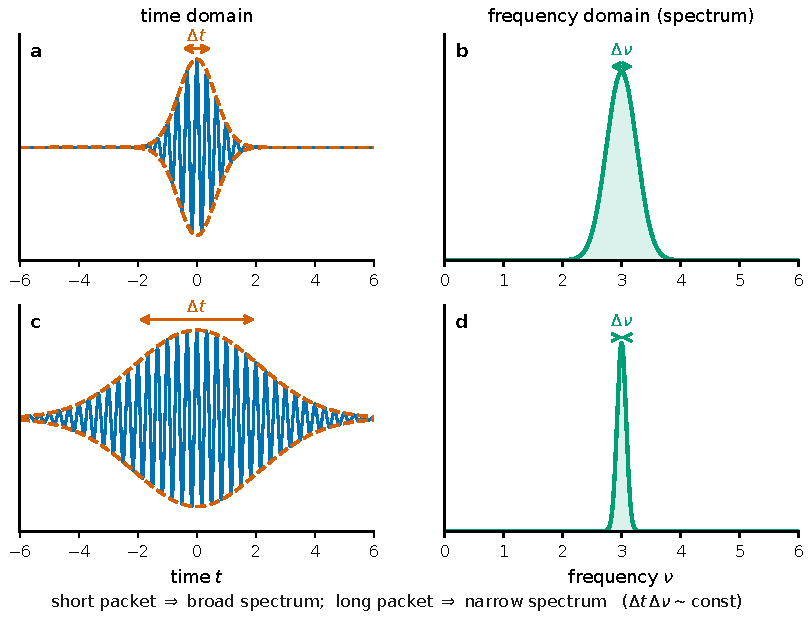
\includegraphics[width=0.9\linewidth]{figures/generated/edu_ch02/e02_wave_packet_spectrum.pdf}
\caption{有限长波包的"时间—频率互易"。上排是短波包：时间上被掐得很窄（\(\Delta t\) 小，橙色双箭头），频谱却铺得很宽（\(\Delta\nu\) 大）；下排是长波包：时间上拉得很长，频谱反而挤成一条窄峰。橙色虚线是包络，绿色是对应的频谱。两排的乘积 \(\Delta t\,\Delta\nu\) 都约为同一个常数——这正是式 \eqref{eq:e02-bandwidth-time} 的图像。}
\label{fig:e02-wave-packet}
\end{figure}

\section{把带宽算成真实数字}
\label{sec:e02-bandwidth}

天文观测里，我们通常不是直接知道频率带宽 \(\Delta\nu\)，而是知道滤光片的中心波长 \(\lambda\) 和波长带宽 \(\Delta\lambda\)（比如"500 纳米中心、1 纳米半宽"）。要把它翻成频率带宽，只需对 \(\nu\) 与 \(\lambda\) 的关系做一步微分。频率和波长由光速联系：
\[
  \nu=\frac{c}{\lambda}.
\]
这里 \(c\approx3\times10^{10}\,{\rm cm\,s^{-1}}\) 是光速；沿用全书的 CGS 单位约定，波长 \(\lambda\) 以厘米计、频率 \(\nu\) 以赫兹计。对 \(\lambda\) 求导，这一步不能跳——用 \(\dfrac{d}{d\lambda}\bigl(c\lambda^{-1}\bigr)=-c\lambda^{-2}\)：
\[
  \frac{d\nu}{d\lambda}=-\frac{c}{\lambda^{2}}.
\]
负号表示波长增大时频率减小，这是意料之中的反比关系；我们关心的是带宽的大小，取绝对值，并把微分 \(d\lambda\) 换成有限的小带宽 \(\Delta\lambda\)（只要 \(\Delta\lambda\ll\lambda\)，用微分近似有限差就足够精确）：
\begin{equation}
  \Delta\nu\;\simeq\;\frac{c\,\Delta\lambda}{\lambda^{2}} .
  \label{eq:e02-bandwidth-conversion}
\end{equation}
\begin{formulaexplain}
\(\Delta\nu\) 是频率带宽，\(\Delta\lambda\) 是波长带宽，\(\lambda\) 是中心波长，\(c\) 是光速。同样的 \(\Delta\lambda\)，波长越短（\(\lambda^2\) 越小），换算出的频率带宽越大。
\end{formulaexplain}
注意分母是 \(\lambda^{2}\) 而不是 \(\lambda\)：这提醒我们，同样"1 纳米"的波长窗口，在蓝端对应的频率带宽比红端更大。现在代入真实数字。取一片可见光滤光片，\(\lambda=500\,{\rm nm}=5\times10^{-5}\,{\rm cm}\)，\(\Delta\lambda=1\,{\rm nm}=1\times10^{-7}\,{\rm cm}\)：
\[
  \Delta\nu\simeq
  \frac{(3\times10^{10}\,{\rm cm\,s^{-1}})\times(1\times10^{-7}\,{\rm cm})}
       {(5\times10^{-5}\,{\rm cm})^{2}}
  =\frac{3\times10^{3}}{2.5\times10^{-9}}\,{\rm Hz}
  =1.2\times10^{12}\,{\rm Hz}.
\]
也就是约 \(1.2\,{\rm THz}\)（太赫兹）。请把这个数量级记牢：一片看起来"很窄"的 1 纳米滤光片，在频率上其实放行了一个上万亿赫兹宽的窗口。和载波频率 \(\nu_0\sim6\times10^{14}\,{\rm Hz}\) 相比，这个窗口只占 \(0.2\%\)，光谱学意义上确实"窄"；但换算成时间尺度以后，它会带来一个惊人的短。这正是下一节的主角。

\section{相干时间：波还记得自己相位多久}
\label{sec:e02-coherence-time}

现在把上一节的带宽翻译成时间。回到铁律 \eqref{eq:e02-bandwidth-time}：一段频率铺开 \(\Delta\nu\) 的光，在时间上最多只能保持约 \(\Delta t\sim1/\Delta\nu\) 的"协调"。给这个时间起个名字，叫\textbf{相干时间}（coherence time）\(\tau_c\)：
\begin{equation}
  \tau_c\;\simeq\;\frac{1}{\Delta\nu}
  \;\simeq\;\frac{\lambda^{2}}{c\,\Delta\lambda} .
  \label{eq:e02-coherence-time}
\end{equation}
\begin{formulaexplain}
\(\tau_c\) 是相干时间，单位秒；带宽 \(\Delta\nu\) 越宽，相干时间越短。第二个等号只是把式 \eqref{eq:e02-bandwidth-conversion} 代进来，用波长量表达。它是光"记得自己相位"的时长，不是探测器的时间分辨率。
\end{formulaexplain}
怎么理解 \(\tau_c\)？把光想成那支旋转的复振幅箭头。如果光是理想单频的，箭头就以恒定角速度匀速转，你只要看一眼此刻的指向，就能准确预言一微秒后、一小时后它指向哪里——它"永远记得"自己的相位。可真实的光有带宽：里面混着一大堆频率略有差别的箭头，它们转速稍有快慢，一开始还整齐，转着转着就散开了，合成箭头的相位越来越不可预测。\(\tau_c\) 就是"从整齐到散乱"所需的时间——过了 \(\tau_c\)，光基本已经忘了自己 \(\tau_c\) 之前的相位。带宽越宽，混进来的转速差别越大，忘得越快。

代入上一节的数字，\(\Delta\nu\simeq1.2\times10^{12}\,{\rm Hz}\)：
\[
  \tau_c\simeq\frac{1}{1.2\times10^{12}\,{\rm Hz}}
  \approx8.3\times10^{-13}\,{\rm s}
  \approx0.8\,{\rm ps}.
\]
不到一皮秒（picosecond，\(1\,{\rm ps}=10^{-12}\,{\rm s}\)）。这就是那片"很窄"的 1 纳米滤光片给出的相干时间：光只能记住自己的相位约 0.8 皮秒，然后就翻篇了。

这个数字之所以要用整章去准备，是因为它和探测器的能力之间有一道触目惊心的鸿沟。最快的单光子探测器（雪崩光电二极管 APD、光电倍增管 PMT）的时间响应大约在 100 皮秒到 1 纳秒之间。拿相干时间去比：
\[
  \frac{\Delta t_{\rm det}}{\tau_c}\sim
  \frac{100\,{\rm ps}\;\text{到}\;1\,{\rm ns}}{0.8\,{\rm ps}}
  \approx1.2\times10^{2}\;\text{到}\;1.2\times10^{3}.
\]
也就是说，探测器一个时间门（time bin）的宽度，是相干时间的\emph{成百上千倍}。换句话说，你每记录一个时间门的强度，其实是把成百上千段互不相干、各自独立的波列平均在了一起。探测器根本来不及看清任何单独一段波列的相位起伏；它看到的永远是一大堆相干时间被抹平后的平均能量。这个结论——"一个时间门里平均了 \(N\sim10^{2}\)--\(10^{3}\) 个相干时间"——会在后面讲光子统计、聚束、强度干涉时反复登场，并直接决定我们能测到的信号被稀释多少倍。

\begin{figure}[tbp]
\centering
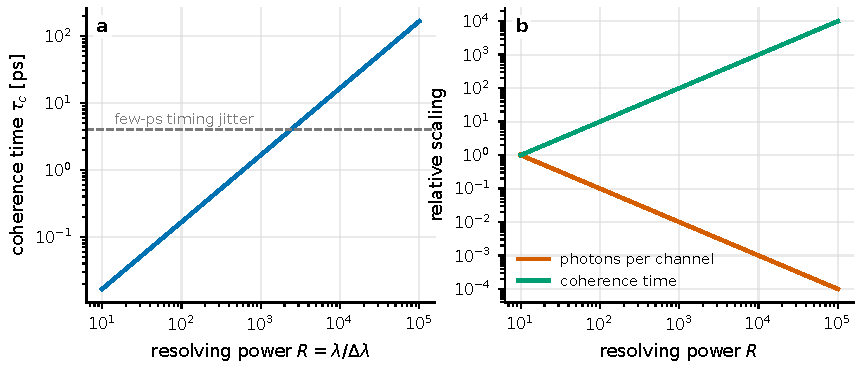
\includegraphics[width=0.85\linewidth]{figures/generated/chapter_06/ch06_spectral_resolution_coherence.pdf}
\caption{光谱分辨率与相干时间是同一件事的两面。谱线（带宽 \(\Delta\nu\)）越窄，对应的相干时间 \(\tau_c\simeq1/\Delta\nu\) 越长；反之宽带光的相干时间极短。图中把可见光宽带滤光片给出的 ps 量级 \(\tau_c\) 与探测器的 100\,ps--1\,ns 响应放在一起，可见一个时间门内包含了大量互不相干的波列。}
\label{fig:e02-spectral-coherence}
\end{figure}

小结一句：带宽和相干时间是同一枚硬币的两面，\(\tau_c\simeq1/\Delta\nu\)。可见光宽带下 \(\tau_c\) 短到皮秒，而探测器慢到百皮秒以上，二者相差百倍以上——这道鸿沟是后面一切强度测量的背景板。

\section{自相关与功率谱：走向相干函数}
\label{sec:e02-autocorrelation}

前面我们用"\(\tau_c\) 是相位记忆的时长"来描述相干时间，那是个定性说法。怎么把"记忆"量化成一条可计算、可测量的曲线？答案是\textbf{自相关函数}（autocorrelation function）。它的想法极其朴素：把信号和"延迟了 \(\tau\) 的自己"相乘再取平均，看它们还有多像。对一个（平稳的）信号 \(f(t)\)，定义
\begin{equation}
  \Gamma(\tau)=\bigl\langle f^{*}(t)\,f(t+\tau)\bigr\rangle
  =\lim_{T\to\infty}\frac{1}{T}\int_{0}^{T} f^{*}(t)\,f(t+\tau)\,dt ,
  \label{eq:e02-autocorrelation}
\end{equation}
\begin{formulaexplain}
\(\Gamma(\tau)\) 是自相关函数；\(\tau\) 是时间延迟；尖括号（或时间积分）表示对时间取平均；\(f^*\) 是复共轭。它衡量"信号此刻"与"信号在 \(\tau\) 之后"的相似程度。
\end{formulaexplain}
当延迟 \(\tau=0\) 时，\(\Gamma(0)=\langle|f|^{2}\rangle\) 就是信号的平均强度（正实数、最大值）。随着 \(\tau\) 增大，如果信号还"记得"自己，\(f^*(t)\) 与 \(f(t+\tau)\) 的相位仍步调一致，乘积平均后不会相消，\(\Gamma\) 保持较大；一旦 \(\tau\) 超过相干时间，两者相位早已各走各的、随机分布，正负乘积在平均中相互抵消，\(\Gamma\to0\)。所以\emph{自相关函数从峰值衰减到零的宽度，正是相干时间 \(\tau_c\)}。这就把上一节那个含糊的"记忆时长"变成了一条曲线的宽度——可算、可测。图~\ref{fig:e02-coherence} 左图正展示了这种衰减：带宽越宽，归一化的自相关掉得越快、相干时间越短；右图把 \(\tau_c\simeq1/\Delta\nu\) 这条标度画成了一条直线。

\begin{figure}[tbp]
\centering
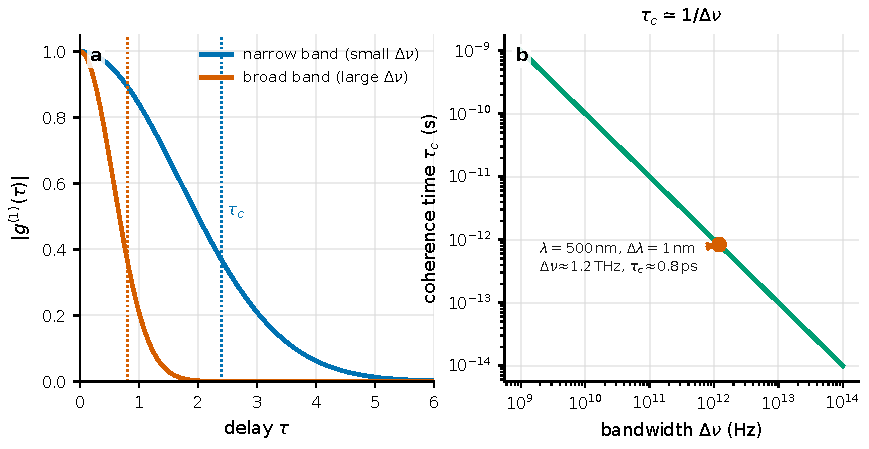
\includegraphics[width=0.92\linewidth]{figures/generated/edu_ch02/e02_coherence_bandwidth.pdf}
\caption{相干时间与带宽互为倒数。左：归一化自相关（也就是后面要正式定义的一阶相干度 \(|g^{(1)}(\tau)|\)）随延迟 \(\tau\) 衰减；带宽越宽（橙）掉得越快、相干时间 \(\tau_c\) 越短，带宽越窄（蓝）则"记得"越久。右：\(\tau_c\simeq1/\Delta\nu\) 在双对数坐标下是一条直线，橙点标出 \(500\,{\rm nm}\)、\(1\,{\rm nm}\) 滤光片给出的 \(\Delta\nu\approx1.2\,{\rm THz}\)、\(\tau_c\approx0.8\,{\rm ps}\)。}
\label{fig:e02-coherence}
\end{figure}

最后要点出一个漂亮而深刻的定理，它把本章两条主线（频谱与相干）系成一个结。这就是\textbf{维纳–辛钦定理}（Wiener–Khinchin theorem）：信号的\textbf{功率谱}（power spectrum）\(S(\nu)\)，恰好是它的自相关函数的傅里叶变换：
\begin{equation}
  S(\nu)=\int_{-\infty}^{+\infty}\Gamma(\tau)\,e^{-\,i\,2\pi\nu\tau}\,d\tau .
  \label{eq:e02-wiener-khinchin}
\end{equation}
\begin{formulaexplain}
\(S(\nu)\) 是功率谱，告诉你各频率占多少功率；\(\Gamma(\tau)\) 是自相关函数。二者是一对傅里叶变换。"信号里有哪些频率"与"信号记得自己多久"是同一件事的两种说法。
\end{formulaexplain}
这个定理的含义值得慢慢体会。它说：\emph{你不必真的去测频谱，只要测出自相关函数，做一次傅里叶变换就得到功率谱；反过来也一样}。这正是式 \eqref{eq:e02-bandwidth-time} 的严格化身——自相关的宽度（相干时间 \(\tau_c\)）与功率谱的宽度（带宽 \(\Delta\nu\)）是一对傅里叶伙伴，一个窄另一个必宽，乘积约为 1。回头看高斯波包那节：时间高斯和频率高斯互为傅里叶变换、宽度成反比，正是维纳–辛钦定理的一个具体样本。

为什么在一本天文书里要这么郑重其事地介绍自相关？因为式 \eqref{eq:e02-autocorrelation} 里那个 \(\langle f^*(t)f(t+\tau)\rangle\) 的结构，几乎原封不动就是后面要定义的\textbf{一阶相干函数}（first-order coherence function）\(g^{(1)}(\tau)\)——只要把 \(f\) 换成电场，再归一化。也就是说，本章的自相关函数就是相干函数的"经典彩排"。等我们在第 \ref{chap:e05} 章之后正式引入 \(g^{(1)}\) 和 \(g^{(2)}\) 时，你会发现它们并不神秘：\(g^{(1)}\) 量的就是电场的自相关（相位记忆），它的宽度就是这里的 \(\tau_c\)；而恒星的谱线形状与它之间，正由维纳–辛钦定理这座桥连接。本章搭好的这套语言——频谱、带宽、相干时间、自相关——就是整本相干理论的地基。

\section{本章要点}
\label{sec:e02-summary}

\begin{itemize}
  \item \textbf{傅里叶思想}：任何波都是纯音的叠加。周期信号给离散谐波（傅里叶级数），非周期信号给连续频谱（傅里叶变换，式 \eqref{eq:e02-fourier-transform}）。频谱就是"每个频率占多少份量"的清单。
  \item \textbf{时间—频率互易}：波列越短，频率越宽，\(\Delta\nu\,\Delta t\gtrsim1\)（式 \eqref{eq:e02-bandwidth-time}）。高斯波包取到最紧凑的下限 \(\sigma_t\sigma_\nu=1/2\pi\)，且其傅里叶变换仍是高斯。
  \item \textbf{带宽换算}：由 \(\nu=c/\lambda\) 微分得 \(\Delta\nu\simeq c\,\Delta\lambda/\lambda^{2}\)。500\,nm、1\,nm 滤光片给 \(\Delta\nu\approx1.2\times10^{12}\,{\rm Hz}\)。
  \item \textbf{相干时间}：\(\tau_c\simeq1/\Delta\nu\approx0.8\,{\rm ps}\)。它是光记得自己相位的时长。探测器 100\,ps--1\,ns 的响应比它长百到千倍——一个时间门平均了成百上千个相干时间。
  \item \textbf{自相关与功率谱}：自相关 \(\Gamma(\tau)\) 的衰减宽度就是 \(\tau_c\)；维纳–辛钦定理（式 \eqref{eq:e02-wiener-khinchin}）说功率谱是自相关的傅里叶变换。这正是一阶相干函数 \(g^{(1)}\) 的前身。
\end{itemize}

\noindent\textbf{想一想}：
\begin{enumerate}
  \item 如果把滤光片换成 \(10\,{\rm nm}\) 带宽，相干时间会变成多少？探测器一个 \(1\,{\rm ns}\) 时间门里又平均了多少个相干时间？
  \item 一列被碰撞平均每 \(\tau_c\) 打断一次的波列，它的谱线大约有多宽？（提示：用式 \eqref{eq:e02-bandwidth-time} 反推。）
  \item 为什么说"测自相关函数"和"测光谱"在信息上是等价的？维纳–辛钦定理在其中扮演什么角色？
\end{enumerate}
